% credits for the pictures made by unknown sources.
% this document was summarised by cos.

\documentclass[letterpaper,10pt,addpoints]{exam}
\usepackage[utf8]{inputenc}
\usepackage[english]{babel}

\usepackage[top=1in, bottom=1in, left=0.75in, right=0.75in]{geometry}
\usepackage{amsmath,amssymb}
\usepackage{graphicx}


\newcommand{\content}{2003 National Higher Education Entrance Examination\\(national version)\\\bigskip \textbf{Mathematics}\\ (Science, engineering, agriculture and medicine)}
\newcommand{\examdate}{2003/06/07 15:00 - 17:00}
\newcommand{\timelimit}{120 minutes}
\author{}

\pagestyle{headandfoot}
\firstpageheader{}{}{}

\begin{document}

\vspace*{\fill}
\begin{center}
\begin{minipage}{\textwidth}
\title{\Large \content}
\date{\examdate\\ \timelimit}
\maketitle

\noindent \rule{\textwidth}{1pt}

\noindent This exam is composed by \textbf{Part I} (multiple choice) and \textbf{Part II} (non-multiple choice). Please return both this exam and answer sheet after the exam period is finished.
\end{minipage}
\end{center}
\vfill 




\clearpage
\begin{center}
\section*{Part I (60 points)}
\end{center}
\subsection*{1. MULTIPLE CHOICES}
\large{\textbf{This section consists of 12 questions. Each question is worth 5 points and there are 60 points available. Only one option is correct for each question.}\\}
\noindent \rule{\textwidth}{1pt}

\begin{questions}
\question
Given that $x\in (-\frac{\pi}{2},0)$, $\cos x=\frac{4}{5}$, then $\tan 2x$ is
\begin{choices}
\choice $\frac{7}{24}$
\choice $-\frac{7}{24}$
\choice $\frac{24}{7}$
\choice $-\frac{24}{7}$
\end{choices}

\question
The directrix of the conic section $\rho=\frac{8\sin\theta}{\cos^2\theta}$ is
\begin{choices}
\choice $\rho\cos\theta=-2$
\choice $\rho\cos\theta=2$
\choice $\rho\sin\theta=2$
\choice $\rho\sin\theta=-2$
\end{choices}

\question
Set the function $f(x)=\begin{cases}
2^{-x}-1, & x\leq 0 \\ 
x^{\frac{1}{2}}, & x>0 
\end{cases}$. If $f(x_0)>1$, then the range of $x_0$ is
\begin{choices}
\choice $(-1,1)$
\choice $(-1,+\infty)$
\choice $(-\infty,-2)\cup (0,+\infty)$
\choice $(-\infty,-1)\cup(1,+\infty)$
\end{choices}

\question
The maximum of the function $y=2\sin x(\sin x+\cos x)$ is
\begin{choices}
\choice $1+\sqrt{2}$
\choice $\sqrt{2}-1$
\choice $\sqrt{2}$
\choice $2$
\end{choices}

\question
Given a circle $C$: $(x-a)^{2}+(y-2)^{2}=4\,(a>0)$ and a line $l$: $x-y+3=0$, when the chore determined by intersecting $C$ by $l$ has length $2\sqrt{3}$, $a$ should be
\begin{choices}
\choice $\sqrt{2}$
\choice $2-\sqrt{2}$
\choice $\sqrt{2}-1$
\choice $\sqrt{2}+1$
\end{choices}

\question
Given a cone with bottom radius $R$ and height $3R$, for all its inscribed cylinders, the maximum surface area is
\begin{choices}
\choice $2\pi R^{2}$
\choice $\frac{9}{4} \pi R^{2}$
\choice $\frac{8}{3} \pi R^{2}$
\choice $\frac{3}{2} \pi R^{2}$
\end{choices}

\question
Given that the four roots of the equation $\left(x^{2}-2 x+m\right)\left(x^{2}-2 x+n\right)=0$ form an arithmetic sequence with the first term $\frac{1}{4}$, then $|m-n|$ is
\begin{choices}
\choice $1$
\choice $\frac{3}{4}$
\choice $\frac{1}{2}$
\choice $\frac{3}{8}$
\end{choices}

\question
Suppose a hyperbola is centered at the origin and one of its focuses is $F(\sqrt{7},0)$. A line $y=x-1$ intersects the hyperbola at points $M$ and $N$. The x-axis of the midpoint of $MN$ is $-\frac{2}{3}$. Then the equation for this hyperbola is
\begin{choices}
\choice $\frac{x^{2}}{3}-\frac{y^{2}}{4}=1$
\choice $\frac{x^{2}}{4}-\frac{y^{2}}{3}=1$
\choice $\frac{x^{2}}{5}-\frac{y^{2}}{2}=1$
\choice $\frac{x^{2}}{2}-\frac{y^{2}}{5}=1$
\end{choices}

\question
The inverse, $f^{-1}(x)$, of the function $f(x)=\sin x, x \in\left[\frac{\pi}{2}, \frac{3 \pi}{2}\right]$ is
\begin{choices}
\choice $-\arcsin x,x \in[-1,1]$
\choice $-\pi-\arcsin x,x \in[-1,1]$
\choice $\pi+\arcsin x,x \in[-1,1]$
\choice $\pi-\arcsin x,x \in[-1,1]$
\end{choices}

\question
A rectangle has four vertexes $A(0,0)$, $B(2,0)$, $C(2,1)$ and $D(0,1)$. A point mass, from $P_0$, the midpoint of $AB$, along $\theta$, the angle between itself and $AB$, goes to the point $P_1$ on $BC$. It is then reflected to $CD$, $DA$ and $AB$ on points $P_2$, $P_3$ and $P_4$ (the angle of incident equals to that of reflection). Let the coordinate of $P_4$ be $(x_4,0)$. If $1<x_{4}<2$, then the range of $\tan\theta$ is
\begin{choices}
\choice $\left(\frac{1}{3}, 1\right)$
\choice $\left(\frac{1}{3}, \frac{2}{3}\right)$
\choice $\left(\frac{2}{5}, \frac{1}{2}\right)$
\choice $\left(\frac{2}{5}, \frac{2}{3}\right)$
\end{choices}

\question
$\displaystyle \lim _{n \rightarrow \infty} \frac{C_{2}^{2}+C_{3}^{2}+C_{4}^{2}+\cdots+C_{n}^{2}}{n\left(C_{2}^{1}+C_{3}^{1}+C_{4}^{1}+\cdots+C_{n}^{1}\right)}=$
\begin{choices}
\choice $3$
\choice $\frac{1}{3}$
\choice $\frac{1}{6}$
\choice $6$
\end{choices}

\question
A tetrahedron has all of its edge length equal to $\sqrt{2}$. The four vertexes are all on the same sphere surface, then the surface area of the sphere is
\begin{choices}
\choice $3\pi$
\choice $4\pi$
\choice $3\sqrt{3}\pi$
\choice $6\pi$
\end{choices}

\xdef\mycounter1{\arabic{question}}
\end{questions}
\clearpage

\begin{center}
\section*{Part II (90 points)}
\end{center}
\subsection*{2. SHORT ANSWER}
\large{\textbf{This section consists of 4 questions. Each question is worth 4 points and there are 16 points available. Fill in the answers in the blank area.}\\}
\noindent \rule{\textwidth}{1pt}

\begin{questions}
\setcounter{question}{\mycounter1}

\question
Find the term containing $x^9$ in the expansion of $\left(x^{2}-\frac{1}{2 x}\right)^{9}$: \rule{80pt}{0.5pt}

\question
The range of $x$ that makes the inequality $\log _{2}(-x)<x+1$ hold is: \rule{80pt}{0.5pt}

\question
A region is divided into 5 districts. We colour the map and demand that neighbours do not share the same colour. If we have 4 colours, then there are \rule{80pt}{0.5pt} different colouring schemes. (answer in numbers)
\begin{center}
     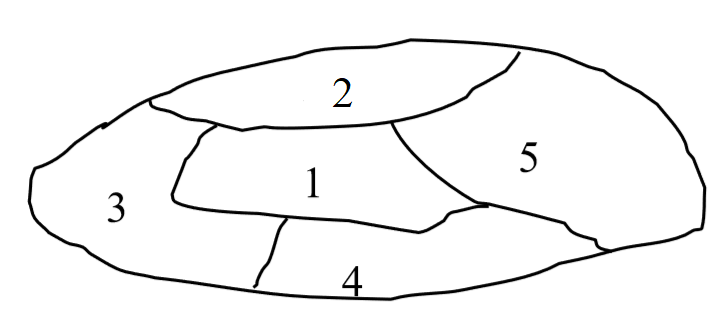
\includegraphics[scale=0.35]{q15.png}
\end{center}

\question
For the following 5 cubes, $l$ is a diagonal and points $M$, $N$, $P$ are at the centers of the edges. The diagrams that have the relation $l\perp \textrm{surface }MNP$ are \rule{80pt}{0.5pt}. (write down all labels)
\begin{center}
    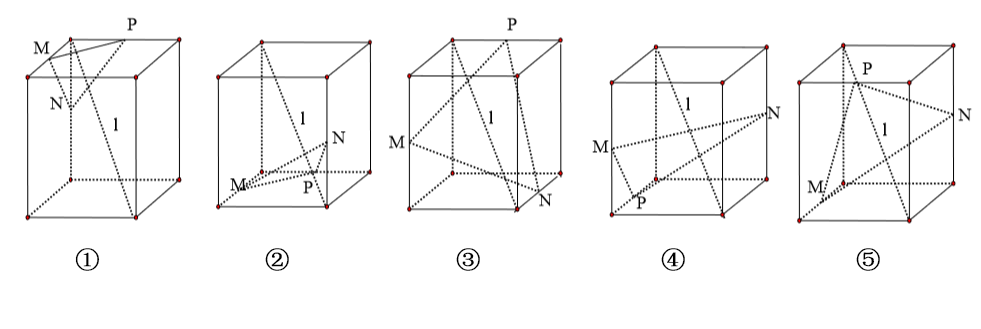
\includegraphics[scale=0.65]{q16.png}
    \end{center}

\xdef\mycounter2{\arabic{question}}
\end{questions}
\clearpage

\subsection*{3. LONG ANSWER}
\large{\textbf{This section consists of 6 questions and there are 74 points available. Candidates should write down their descriptions, proofs or steps.}\\}
\noindent \rule{\textwidth}{1pt}

\begin{questions}
\setcounter{question}{\mycounter2}

\question[12]
Given that the argument of the complex number $z$ is $60^{\circ}$ and that $|z-1|$ is the middle term of the geometric terms $|z|$ and $|z-2|$, find $|z|$.

\question[12]
In the below triangular prism $ABC-A_1B_1C_1$, the base is a isosceles right triangle, $\angle ACB=90^\circ$, the edge $AA_1=2$, $D$ and $E$ are the midpoints of $CC_1$ and $A_1B$, respectively, and the projection of point $E$ onto surface $ABD$ is the centroid $G$ of $\triangle ABC$.
\begin{center}
    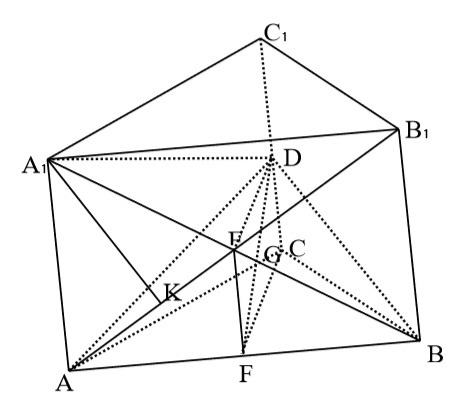
\includegraphics[scale=0.7]{q18.png}
\end{center}
\renewcommand{\labelenumi}{(\Roman{enumi})}
\begin{enumerate}
    \item Find the angle between $A_1B$ and surface $ABD$. (express the answer in inverse trigonometric values)
    \item Find the distance between point $A_1$ and surface $AED$.
\end{enumerate}

\question[12]
Given that $c>0$, let
\renewcommand{\labelenumi}{}
\begin{enumerate}
     \item $P$:= the function $y=c^x$ is monotone decreasing in $\mathbb{R}$.
     \item $Q$:= the inequality $x+|x-2c|>1$ has $\mathbb{R}$ as its solution.
\end{enumerate}
If one and only one of $P$ and $Q$ is correct, find the range of $c$.
\clearpage

\question[12]
A typhoon is spotted on the sea near to a coastal town. According to the observation, the eye of the typhoon is located at east $\theta=\arccos\frac{\sqrt{2}}{10}$ to the south, 300 km away, at the point $P$, relative to the town and is moving west $45^{\circ}$ to the north at a speed of 20 km/h. The range of the typhoon is a circle and has a radius of 60 km which is expanding at a speed of 10 km/h. After how many hours will the town be affected by the typhoon?
\begin{center}
    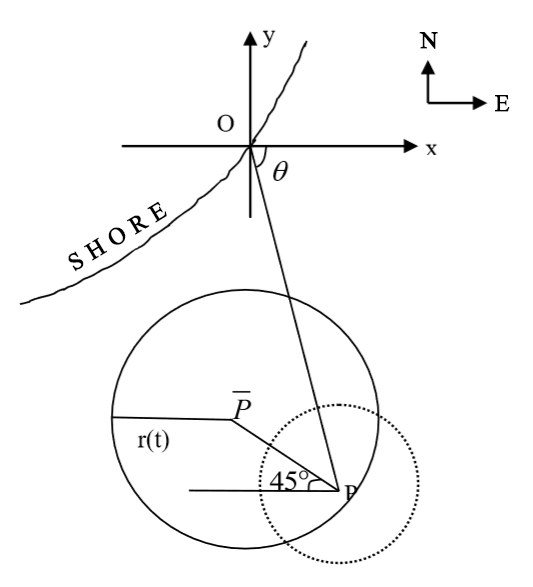
\includegraphics[scale=0.6]{q20.PNG}
\end{center}

\question[14]
Let $a>0$, in the rectangle $ABCD$, $AB=4$, $BC=4a$, $O$ is the midpoint of $AB$, points $E$, $F$, $G$ are moving on $BC$, $CD$, $DA$, respectively, also $\frac{BE}{BC}=\frac{CF}{CD}=\frac{DC}{DA}$, and $P$ is the intersection of $GE$ and $OF$. Do there exist two fixed points such that the sum of their distances to $P$ is a constant? If there are, find the coordinates and such constants of these two points, otherwise explain why they do not exist.
\begin{center}
    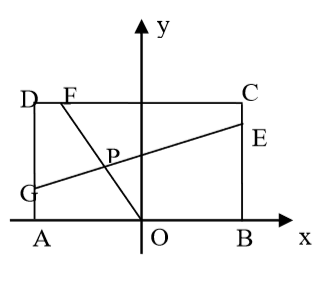
\includegraphics[scale=0.6]{q21.PNG}
\end{center}
\clearpage

\question[12]
\renewcommand{\labelenumi}{(\Roman{enumi})}
\renewcommand{\labelenumii}{(\arabic{enumii})}
\begin{enumerate}
    \item Suppose that $\left\{a_{n}\right\}$ is a sequence formed by rearranging all numbers in the set $\left\{2^{s}+2^{t} \,|\, 0 \leq s<t \textrm{ and } s, t \in \mathbb{Z}\right\}$ in increasing order, i.e. $a_{1}=3, a_{2}=5, a_{3}=6, a_{4}=9, a_{5}=10, a_{6}=12, \ldots$ \\
    Now write $\left\{a_{n}\right\}$ as a triangular number array based on: 1. the smaller is on the top and the bigger on the bottom 2. the smaller is on the left and the bigger on the right.
    \begin{center}
        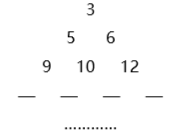
\includegraphics[scale=0.8]{q22.PNG}
    \end{center}
    \begin{enumerate}
        \item Write down the numbers on the fourth and fifth rows of this array.
        \item Find $a_{100}$.
    \end{enumerate}
    \item (This item is a bonus question. If it is answered correctly, 4 points are added to the exam, but the total score should not exceed 150) Let $\left\{b_{n}\right\}$ be the sequence formed by rearranging all numbers in the set $\left\{2^{r}+2^{s}+2^{t} \,|\, 0 \leq r<s<t \textrm{ and } r, s, t \in \mathbb{Z}\right\}$ in increasing order. Given that $b_k=1160$, find $k$.
\end{enumerate}

\end{questions}
\end{document}